% Created by tikzDevice version 0.10.1 on 2017-11-26 21:02:45
% !TEX encoding = UTF-8 Unicode
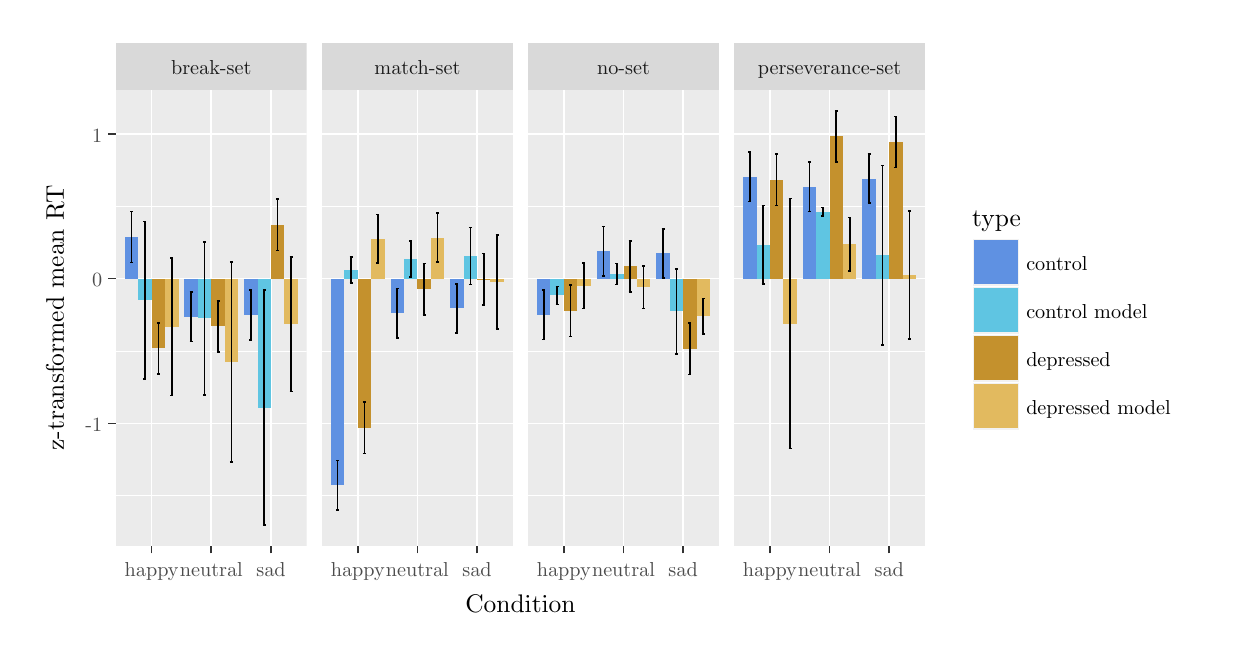
\begin{tikzpicture}[x=1pt,y=1pt]
\definecolor{fillColor}{RGB}{255,255,255}
\path[use as bounding box,fill=fillColor,fill opacity=0.00] (0,0) rectangle (433.62,216.81);
\begin{scope}
\path[clip] (  0.00,  0.00) rectangle (433.62,216.81);
\definecolor{drawColor}{RGB}{255,255,255}
\definecolor{fillColor}{RGB}{255,255,255}

\path[draw=drawColor,line width= 0.6pt,line join=round,line cap=round,fill=fillColor] (  0.00,  0.00) rectangle (433.62,216.81);
\end{scope}
\begin{scope}
\path[clip] ( 31.87, 29.59) rectangle (100.84,194.25);
\definecolor{fillColor}{gray}{0.92}

\path[fill=fillColor] ( 31.87, 29.59) rectangle (100.84,194.25);
\definecolor{drawColor}{RGB}{255,255,255}

\path[draw=drawColor,line width= 0.3pt,line join=round] ( 31.87, 47.66) --
	(100.84, 47.66);

\path[draw=drawColor,line width= 0.3pt,line join=round] ( 31.87, 99.99) --
	(100.84, 99.99);

\path[draw=drawColor,line width= 0.3pt,line join=round] ( 31.87,152.32) --
	(100.84,152.32);

\path[draw=drawColor,line width= 0.6pt,line join=round] ( 31.87, 73.82) --
	(100.84, 73.82);

\path[draw=drawColor,line width= 0.6pt,line join=round] ( 31.87,126.15) --
	(100.84,126.15);

\path[draw=drawColor,line width= 0.6pt,line join=round] ( 31.87,178.48) --
	(100.84,178.48);

\path[draw=drawColor,line width= 0.6pt,line join=round] ( 44.80, 29.59) --
	( 44.80,194.25);

\path[draw=drawColor,line width= 0.6pt,line join=round] ( 66.36, 29.59) --
	( 66.36,194.25);

\path[draw=drawColor,line width= 0.6pt,line join=round] ( 87.91, 29.59) --
	( 87.91,194.25);
\definecolor{fillColor}{RGB}{226,186,95}

\path[fill=fillColor] ( 49.65,108.73) rectangle ( 54.50,126.15);
\definecolor{fillColor}{RGB}{196,145,45}

\path[fill=fillColor] ( 44.80,100.92) rectangle ( 49.65,126.15);
\definecolor{fillColor}{RGB}{95,197,226}

\path[fill=fillColor] ( 39.95,118.30) rectangle ( 44.80,126.15);
\definecolor{fillColor}{RGB}{95,145,226}

\path[fill=fillColor] ( 35.10,126.15) rectangle ( 39.95,141.17);
\definecolor{fillColor}{RGB}{226,186,95}

\path[fill=fillColor] ( 71.21, 95.99) rectangle ( 76.06,126.15);
\definecolor{fillColor}{RGB}{196,145,45}

\path[fill=fillColor] ( 66.36,108.88) rectangle ( 71.21,126.15);
\definecolor{fillColor}{RGB}{95,197,226}

\path[fill=fillColor] ( 61.51,111.72) rectangle ( 66.36,126.15);
\definecolor{fillColor}{RGB}{95,145,226}

\path[fill=fillColor] ( 56.66,112.38) rectangle ( 61.51,126.15);
\definecolor{fillColor}{RGB}{226,186,95}

\path[fill=fillColor] ( 92.76,109.59) rectangle ( 97.61,126.15);
\definecolor{fillColor}{RGB}{196,145,45}

\path[fill=fillColor] ( 87.91,126.15) rectangle ( 92.76,145.56);
\definecolor{fillColor}{RGB}{95,197,226}

\path[fill=fillColor] ( 83.06, 79.53) rectangle ( 87.91,126.15);
\definecolor{fillColor}{RGB}{95,145,226}

\path[fill=fillColor] ( 78.21,112.97) rectangle ( 83.06,126.15);
\definecolor{drawColor}{RGB}{0,0,0}

\path[draw=drawColor,line width= 0.6pt,line join=round] ( 51.54,133.50) --
	( 52.62,133.50);

\path[draw=drawColor,line width= 0.6pt,line join=round] ( 52.08,133.50) --
	( 52.08, 83.95);

\path[draw=drawColor,line width= 0.6pt,line join=round] ( 51.54, 83.95) --
	( 52.62, 83.95);

\path[draw=drawColor,line width= 0.6pt,line join=round] ( 46.69,110.21) --
	( 47.77,110.21);

\path[draw=drawColor,line width= 0.6pt,line join=round] ( 47.23,110.21) --
	( 47.23, 91.63);

\path[draw=drawColor,line width= 0.6pt,line join=round] ( 46.69, 91.63) --
	( 47.77, 91.63);

\path[draw=drawColor,line width= 0.6pt,line join=round] ( 41.84,146.72) --
	( 42.92,146.72);

\path[draw=drawColor,line width= 0.6pt,line join=round] ( 42.38,146.72) --
	( 42.38, 89.88);

\path[draw=drawColor,line width= 0.6pt,line join=round] ( 41.84, 89.88) --
	( 42.92, 89.88);

\path[draw=drawColor,line width= 0.6pt,line join=round] ( 36.99,150.34) --
	( 38.07,150.34);

\path[draw=drawColor,line width= 0.6pt,line join=round] ( 37.53,150.34) --
	( 37.53,132.00);

\path[draw=drawColor,line width= 0.6pt,line join=round] ( 36.99,132.00) --
	( 38.07,132.00);

\path[draw=drawColor,line width= 0.6pt,line join=round] ( 73.09,132.17) --
	( 74.17,132.17);

\path[draw=drawColor,line width= 0.6pt,line join=round] ( 73.63,132.17) --
	( 73.63, 59.82);

\path[draw=drawColor,line width= 0.6pt,line join=round] ( 73.09, 59.82) --
	( 74.17, 59.82);

\path[draw=drawColor,line width= 0.6pt,line join=round] ( 68.24,118.14) --
	( 69.32,118.14);

\path[draw=drawColor,line width= 0.6pt,line join=round] ( 68.78,118.14) --
	( 68.78, 99.61);

\path[draw=drawColor,line width= 0.6pt,line join=round] ( 68.24, 99.61) --
	( 69.32, 99.61);

\path[draw=drawColor,line width= 0.6pt,line join=round] ( 63.39,139.38) --
	( 64.47,139.38);

\path[draw=drawColor,line width= 0.6pt,line join=round] ( 63.93,139.38) --
	( 63.93, 84.05);

\path[draw=drawColor,line width= 0.6pt,line join=round] ( 63.39, 84.05) --
	( 64.47, 84.05);

\path[draw=drawColor,line width= 0.6pt,line join=round] ( 58.54,121.31) --
	( 59.62,121.31);

\path[draw=drawColor,line width= 0.6pt,line join=round] ( 59.08,121.31) --
	( 59.08,103.44);

\path[draw=drawColor,line width= 0.6pt,line join=round] ( 58.54,103.44) --
	( 59.62,103.44);

\path[draw=drawColor,line width= 0.6pt,line join=round] ( 94.65,133.88) --
	( 95.72,133.88);

\path[draw=drawColor,line width= 0.6pt,line join=round] ( 95.18,133.88) --
	( 95.18, 85.30);

\path[draw=drawColor,line width= 0.6pt,line join=round] ( 94.65, 85.30) --
	( 95.72, 85.30);

\path[draw=drawColor,line width= 0.6pt,line join=round] ( 89.80,154.85) --
	( 90.87,154.85);

\path[draw=drawColor,line width= 0.6pt,line join=round] ( 90.33,154.85) --
	( 90.33,136.27);

\path[draw=drawColor,line width= 0.6pt,line join=round] ( 89.80,136.27) --
	( 90.87,136.27);

\path[draw=drawColor,line width= 0.6pt,line join=round] ( 84.95,121.99) --
	( 86.02,121.99);

\path[draw=drawColor,line width= 0.6pt,line join=round] ( 85.48,121.99) --
	( 85.48, 37.07);

\path[draw=drawColor,line width= 0.6pt,line join=round] ( 84.95, 37.07) --
	( 86.02, 37.07);

\path[draw=drawColor,line width= 0.6pt,line join=round] ( 80.10,121.91) --
	( 81.17,121.91);

\path[draw=drawColor,line width= 0.6pt,line join=round] ( 80.64,121.91) --
	( 80.64,104.04);

\path[draw=drawColor,line width= 0.6pt,line join=round] ( 80.10,104.04) --
	( 81.17,104.04);
\end{scope}
\begin{scope}
\path[clip] (106.34, 29.59) rectangle (175.31,194.25);
\definecolor{fillColor}{gray}{0.92}

\path[fill=fillColor] (106.34, 29.59) rectangle (175.31,194.25);
\definecolor{drawColor}{RGB}{255,255,255}

\path[draw=drawColor,line width= 0.3pt,line join=round] (106.34, 47.66) --
	(175.31, 47.66);

\path[draw=drawColor,line width= 0.3pt,line join=round] (106.34, 99.99) --
	(175.31, 99.99);

\path[draw=drawColor,line width= 0.3pt,line join=round] (106.34,152.32) --
	(175.31,152.32);

\path[draw=drawColor,line width= 0.6pt,line join=round] (106.34, 73.82) --
	(175.31, 73.82);

\path[draw=drawColor,line width= 0.6pt,line join=round] (106.34,126.15) --
	(175.31,126.15);

\path[draw=drawColor,line width= 0.6pt,line join=round] (106.34,178.48) --
	(175.31,178.48);

\path[draw=drawColor,line width= 0.6pt,line join=round] (119.27, 29.59) --
	(119.27,194.25);

\path[draw=drawColor,line width= 0.6pt,line join=round] (140.83, 29.59) --
	(140.83,194.25);

\path[draw=drawColor,line width= 0.6pt,line join=round] (162.38, 29.59) --
	(162.38,194.25);
\definecolor{fillColor}{RGB}{226,186,95}

\path[fill=fillColor] (124.12,126.15) rectangle (128.97,140.51);
\definecolor{fillColor}{RGB}{196,145,45}

\path[fill=fillColor] (119.27, 72.25) rectangle (124.12,126.15);
\definecolor{fillColor}{RGB}{95,197,226}

\path[fill=fillColor] (114.42,126.15) rectangle (119.27,129.31);
\definecolor{fillColor}{RGB}{95,145,226}

\path[fill=fillColor] (109.57, 51.41) rectangle (114.42,126.15);
\definecolor{fillColor}{RGB}{226,186,95}

\path[fill=fillColor] (145.68,126.15) rectangle (150.53,140.90);
\definecolor{fillColor}{RGB}{196,145,45}

\path[fill=fillColor] (140.83,122.35) rectangle (145.68,126.15);
\definecolor{fillColor}{RGB}{95,197,226}

\path[fill=fillColor] (135.98,126.15) rectangle (140.83,133.28);
\definecolor{fillColor}{RGB}{95,145,226}

\path[fill=fillColor] (131.13,113.63) rectangle (135.98,126.15);
\definecolor{fillColor}{RGB}{226,186,95}

\path[fill=fillColor] (167.23,124.91) rectangle (172.08,126.15);
\definecolor{fillColor}{RGB}{196,145,45}

\path[fill=fillColor] (162.38,125.97) rectangle (167.23,126.15);
\definecolor{fillColor}{RGB}{95,197,226}

\path[fill=fillColor] (157.53,126.15) rectangle (162.38,134.33);
\definecolor{fillColor}{RGB}{95,145,226}

\path[fill=fillColor] (152.68,115.35) rectangle (157.53,126.15);
\definecolor{drawColor}{RGB}{0,0,0}

\path[draw=drawColor,line width= 0.6pt,line join=round] (126.01,149.34) --
	(127.09,149.34);

\path[draw=drawColor,line width= 0.6pt,line join=round] (126.55,149.34) --
	(126.55,131.68);

\path[draw=drawColor,line width= 0.6pt,line join=round] (126.01,131.68) --
	(127.09,131.68);

\path[draw=drawColor,line width= 0.6pt,line join=round] (121.16, 81.51) --
	(122.24, 81.51);

\path[draw=drawColor,line width= 0.6pt,line join=round] (121.70, 81.51) --
	(121.70, 62.99);

\path[draw=drawColor,line width= 0.6pt,line join=round] (121.16, 62.99) --
	(122.24, 62.99);

\path[draw=drawColor,line width= 0.6pt,line join=round] (116.31,133.95) --
	(117.39,133.95);

\path[draw=drawColor,line width= 0.6pt,line join=round] (116.85,133.95) --
	(116.85,124.66);

\path[draw=drawColor,line width= 0.6pt,line join=round] (116.31,124.66) --
	(117.39,124.66);

\path[draw=drawColor,line width= 0.6pt,line join=round] (111.46, 60.37) --
	(112.54, 60.37);

\path[draw=drawColor,line width= 0.6pt,line join=round] (112.00, 60.37) --
	(112.00, 42.44);

\path[draw=drawColor,line width= 0.6pt,line join=round] (111.46, 42.44) --
	(112.54, 42.44);

\path[draw=drawColor,line width= 0.6pt,line join=round] (147.56,149.77) --
	(148.64,149.77);

\path[draw=drawColor,line width= 0.6pt,line join=round] (148.10,149.77) --
	(148.10,132.03);

\path[draw=drawColor,line width= 0.6pt,line join=round] (147.56,132.03) --
	(148.64,132.03);

\path[draw=drawColor,line width= 0.6pt,line join=round] (142.71,131.62) --
	(143.79,131.62);

\path[draw=drawColor,line width= 0.6pt,line join=round] (143.25,131.62) --
	(143.25,113.09);

\path[draw=drawColor,line width= 0.6pt,line join=round] (142.71,113.09) --
	(143.79,113.09);

\path[draw=drawColor,line width= 0.6pt,line join=round] (137.86,139.77) --
	(138.94,139.77);

\path[draw=drawColor,line width= 0.6pt,line join=round] (138.40,139.77) --
	(138.40,126.79);

\path[draw=drawColor,line width= 0.6pt,line join=round] (137.86,126.79) --
	(138.94,126.79);

\path[draw=drawColor,line width= 0.6pt,line join=round] (133.01,122.56) --
	(134.09,122.56);

\path[draw=drawColor,line width= 0.6pt,line join=round] (133.55,122.56) --
	(133.55,104.69);

\path[draw=drawColor,line width= 0.6pt,line join=round] (133.01,104.69) --
	(134.09,104.69);

\path[draw=drawColor,line width= 0.6pt,line join=round] (169.12,141.79) --
	(170.19,141.79);

\path[draw=drawColor,line width= 0.6pt,line join=round] (169.65,141.79) --
	(169.65,108.04);

\path[draw=drawColor,line width= 0.6pt,line join=round] (169.12,108.04) --
	(170.19,108.04);

\path[draw=drawColor,line width= 0.6pt,line join=round] (164.27,135.23) --
	(165.34,135.23);

\path[draw=drawColor,line width= 0.6pt,line join=round] (164.80,135.23) --
	(164.80,116.71);

\path[draw=drawColor,line width= 0.6pt,line join=round] (164.27,116.71) --
	(165.34,116.71);

\path[draw=drawColor,line width= 0.6pt,line join=round] (159.42,144.61) --
	(160.49,144.61);

\path[draw=drawColor,line width= 0.6pt,line join=round] (159.96,144.61) --
	(159.96,124.05);

\path[draw=drawColor,line width= 0.6pt,line join=round] (159.42,124.05) --
	(160.49,124.05);

\path[draw=drawColor,line width= 0.6pt,line join=round] (154.57,124.28) --
	(155.64,124.28);

\path[draw=drawColor,line width= 0.6pt,line join=round] (155.11,124.28) --
	(155.11,106.41);

\path[draw=drawColor,line width= 0.6pt,line join=round] (154.57,106.41) --
	(155.64,106.41);
\end{scope}
\begin{scope}
\path[clip] (180.81, 29.59) rectangle (249.78,194.25);
\definecolor{fillColor}{gray}{0.92}

\path[fill=fillColor] (180.81, 29.59) rectangle (249.78,194.25);
\definecolor{drawColor}{RGB}{255,255,255}

\path[draw=drawColor,line width= 0.3pt,line join=round] (180.81, 47.66) --
	(249.78, 47.66);

\path[draw=drawColor,line width= 0.3pt,line join=round] (180.81, 99.99) --
	(249.78, 99.99);

\path[draw=drawColor,line width= 0.3pt,line join=round] (180.81,152.32) --
	(249.78,152.32);

\path[draw=drawColor,line width= 0.6pt,line join=round] (180.81, 73.82) --
	(249.78, 73.82);

\path[draw=drawColor,line width= 0.6pt,line join=round] (180.81,126.15) --
	(249.78,126.15);

\path[draw=drawColor,line width= 0.6pt,line join=round] (180.81,178.48) --
	(249.78,178.48);

\path[draw=drawColor,line width= 0.6pt,line join=round] (193.74, 29.59) --
	(193.74,194.25);

\path[draw=drawColor,line width= 0.6pt,line join=round] (215.30, 29.59) --
	(215.30,194.25);

\path[draw=drawColor,line width= 0.6pt,line join=round] (236.85, 29.59) --
	(236.85,194.25);
\definecolor{fillColor}{RGB}{226,186,95}

\path[fill=fillColor] (198.59,123.57) rectangle (203.44,126.15);
\definecolor{fillColor}{RGB}{196,145,45}

\path[fill=fillColor] (193.74,114.52) rectangle (198.59,126.15);
\definecolor{fillColor}{RGB}{95,197,226}

\path[fill=fillColor] (188.89,120.03) rectangle (193.74,126.15);
\definecolor{fillColor}{RGB}{95,145,226}

\path[fill=fillColor] (184.05,113.15) rectangle (188.89,126.15);
\definecolor{fillColor}{RGB}{226,186,95}

\path[fill=fillColor] (220.15,122.96) rectangle (225.00,126.15);
\definecolor{fillColor}{RGB}{196,145,45}

\path[fill=fillColor] (215.30,126.15) rectangle (220.15,130.55);
\definecolor{fillColor}{RGB}{95,197,226}

\path[fill=fillColor] (210.45,126.15) rectangle (215.30,127.80);
\definecolor{fillColor}{RGB}{95,145,226}

\path[fill=fillColor] (205.60,126.15) rectangle (210.45,136.01);
\definecolor{fillColor}{RGB}{226,186,95}

\path[fill=fillColor] (241.70,112.56) rectangle (246.55,126.15);
\definecolor{fillColor}{RGB}{196,145,45}

\path[fill=fillColor] (236.85,100.74) rectangle (241.70,126.15);
\definecolor{fillColor}{RGB}{95,197,226}

\path[fill=fillColor] (232.00,114.32) rectangle (236.85,126.15);
\definecolor{fillColor}{RGB}{95,145,226}

\path[fill=fillColor] (227.15,126.15) rectangle (232.00,135.24);
\definecolor{drawColor}{RGB}{0,0,0}

\path[draw=drawColor,line width= 0.6pt,line join=round] (200.48,131.82) --
	(201.56,131.82);

\path[draw=drawColor,line width= 0.6pt,line join=round] (201.02,131.82) --
	(201.02,115.31);

\path[draw=drawColor,line width= 0.6pt,line join=round] (200.48,115.31) --
	(201.56,115.31);

\path[draw=drawColor,line width= 0.6pt,line join=round] (195.63,123.78) --
	(196.71,123.78);

\path[draw=drawColor,line width= 0.6pt,line join=round] (196.17,123.78) --
	(196.17,105.25);

\path[draw=drawColor,line width= 0.6pt,line join=round] (195.63,105.25) --
	(196.71,105.25);

\path[draw=drawColor,line width= 0.6pt,line join=round] (190.78,123.34) --
	(191.86,123.34);

\path[draw=drawColor,line width= 0.6pt,line join=round] (191.32,123.34) --
	(191.32,116.72);

\path[draw=drawColor,line width= 0.6pt,line join=round] (190.78,116.72) --
	(191.86,116.72);

\path[draw=drawColor,line width= 0.6pt,line join=round] (185.93,122.11) --
	(187.01,122.11);

\path[draw=drawColor,line width= 0.6pt,line join=round] (186.47,122.11) --
	(186.47,104.19);

\path[draw=drawColor,line width= 0.6pt,line join=round] (185.93,104.19) --
	(187.01,104.19);

\path[draw=drawColor,line width= 0.6pt,line join=round] (222.03,130.60) --
	(223.11,130.60);

\path[draw=drawColor,line width= 0.6pt,line join=round] (222.57,130.60) --
	(222.57,115.33);

\path[draw=drawColor,line width= 0.6pt,line join=round] (222.03,115.33) --
	(223.11,115.33);

\path[draw=drawColor,line width= 0.6pt,line join=round] (217.18,139.84) --
	(218.26,139.84);

\path[draw=drawColor,line width= 0.6pt,line join=round] (217.72,139.84) --
	(217.72,121.26);

\path[draw=drawColor,line width= 0.6pt,line join=round] (217.18,121.26) --
	(218.26,121.26);

\path[draw=drawColor,line width= 0.6pt,line join=round] (212.33,131.54) --
	(213.41,131.54);

\path[draw=drawColor,line width= 0.6pt,line join=round] (212.87,131.54) --
	(212.87,124.06);

\path[draw=drawColor,line width= 0.6pt,line join=round] (212.33,124.06) --
	(213.41,124.06);

\path[draw=drawColor,line width= 0.6pt,line join=round] (207.48,144.94) --
	(208.56,144.94);

\path[draw=drawColor,line width= 0.6pt,line join=round] (208.02,144.94) --
	(208.02,127.07);

\path[draw=drawColor,line width= 0.6pt,line join=round] (207.48,127.07) --
	(208.56,127.07);

\path[draw=drawColor,line width= 0.6pt,line join=round] (243.59,119.00) --
	(244.66,119.00);

\path[draw=drawColor,line width= 0.6pt,line join=round] (244.12,119.00) --
	(244.12,106.13);

\path[draw=drawColor,line width= 0.6pt,line join=round] (243.59,106.13) --
	(244.66,106.13);

\path[draw=drawColor,line width= 0.6pt,line join=round] (238.74,110.00) --
	(239.81,110.00);

\path[draw=drawColor,line width= 0.6pt,line join=round] (239.28,110.00) --
	(239.28, 91.48);

\path[draw=drawColor,line width= 0.6pt,line join=round] (238.74, 91.48) --
	(239.81, 91.48);

\path[draw=drawColor,line width= 0.6pt,line join=round] (233.89,129.67) --
	(234.96,129.67);

\path[draw=drawColor,line width= 0.6pt,line join=round] (234.43,129.67) --
	(234.43, 98.98);

\path[draw=drawColor,line width= 0.6pt,line join=round] (233.89, 98.98) --
	(234.96, 98.98);

\path[draw=drawColor,line width= 0.6pt,line join=round] (229.04,144.17) --
	(230.12,144.17);

\path[draw=drawColor,line width= 0.6pt,line join=round] (229.58,144.17) --
	(229.58,126.30);

\path[draw=drawColor,line width= 0.6pt,line join=round] (229.04,126.30) --
	(230.12,126.30);
\end{scope}
\begin{scope}
\path[clip] (255.28, 29.59) rectangle (324.25,194.25);
\definecolor{fillColor}{gray}{0.92}

\path[fill=fillColor] (255.28, 29.59) rectangle (324.25,194.25);
\definecolor{drawColor}{RGB}{255,255,255}

\path[draw=drawColor,line width= 0.3pt,line join=round] (255.28, 47.66) --
	(324.25, 47.66);

\path[draw=drawColor,line width= 0.3pt,line join=round] (255.28, 99.99) --
	(324.25, 99.99);

\path[draw=drawColor,line width= 0.3pt,line join=round] (255.28,152.32) --
	(324.25,152.32);

\path[draw=drawColor,line width= 0.6pt,line join=round] (255.28, 73.82) --
	(324.25, 73.82);

\path[draw=drawColor,line width= 0.6pt,line join=round] (255.28,126.15) --
	(324.25,126.15);

\path[draw=drawColor,line width= 0.6pt,line join=round] (255.28,178.48) --
	(324.25,178.48);

\path[draw=drawColor,line width= 0.6pt,line join=round] (268.21, 29.59) --
	(268.21,194.25);

\path[draw=drawColor,line width= 0.6pt,line join=round] (289.77, 29.59) --
	(289.77,194.25);

\path[draw=drawColor,line width= 0.6pt,line join=round] (311.32, 29.59) --
	(311.32,194.25);
\definecolor{fillColor}{RGB}{226,186,95}

\path[fill=fillColor] (273.06,109.90) rectangle (277.91,126.15);
\definecolor{fillColor}{RGB}{196,145,45}

\path[fill=fillColor] (268.21,126.15) rectangle (273.06,161.83);
\definecolor{fillColor}{RGB}{95,197,226}

\path[fill=fillColor] (263.37,126.15) rectangle (268.21,138.38);
\definecolor{fillColor}{RGB}{95,145,226}

\path[fill=fillColor] (258.52,126.15) rectangle (263.37,162.96);
\definecolor{fillColor}{RGB}{226,186,95}

\path[fill=fillColor] (294.62,126.15) rectangle (299.47,138.54);
\definecolor{fillColor}{RGB}{196,145,45}

\path[fill=fillColor] (289.77,126.15) rectangle (294.62,177.50);
\definecolor{fillColor}{RGB}{95,197,226}

\path[fill=fillColor] (284.92,126.15) rectangle (289.77,150.27);
\definecolor{fillColor}{RGB}{95,145,226}

\path[fill=fillColor] (280.07,126.15) rectangle (284.92,159.34);
\definecolor{fillColor}{RGB}{226,186,95}

\path[fill=fillColor] (316.17,126.15) rectangle (321.02,127.38);
\definecolor{fillColor}{RGB}{196,145,45}

\path[fill=fillColor] (311.32,126.15) rectangle (316.17,175.49);
\definecolor{fillColor}{RGB}{95,197,226}

\path[fill=fillColor] (306.47,126.15) rectangle (311.32,134.55);
\definecolor{fillColor}{RGB}{95,145,226}

\path[fill=fillColor] (301.62,126.15) rectangle (306.47,162.30);
\definecolor{drawColor}{RGB}{0,0,0}

\path[draw=drawColor,line width= 0.6pt,line join=round] (274.95,155.04) --
	(276.03,155.04);

\path[draw=drawColor,line width= 0.6pt,line join=round] (275.49,155.04) --
	(275.49, 64.75);

\path[draw=drawColor,line width= 0.6pt,line join=round] (274.95, 64.75) --
	(276.03, 64.75);

\path[draw=drawColor,line width= 0.6pt,line join=round] (270.10,171.09) --
	(271.18,171.09);

\path[draw=drawColor,line width= 0.6pt,line join=round] (270.64,171.09) --
	(270.64,152.57);

\path[draw=drawColor,line width= 0.6pt,line join=round] (270.10,152.57) --
	(271.18,152.57);

\path[draw=drawColor,line width= 0.6pt,line join=round] (265.25,152.49) --
	(266.33,152.49);

\path[draw=drawColor,line width= 0.6pt,line join=round] (265.79,152.49) --
	(265.79,124.27);

\path[draw=drawColor,line width= 0.6pt,line join=round] (265.25,124.27) --
	(266.33,124.27);

\path[draw=drawColor,line width= 0.6pt,line join=round] (260.40,171.89) --
	(261.48,171.89);

\path[draw=drawColor,line width= 0.6pt,line join=round] (260.94,171.89) --
	(260.94,154.02);

\path[draw=drawColor,line width= 0.6pt,line join=round] (260.40,154.02) --
	(261.48,154.02);

\path[draw=drawColor,line width= 0.6pt,line join=round] (296.50,148.26) --
	(297.58,148.26);

\path[draw=drawColor,line width= 0.6pt,line join=round] (297.04,148.26) --
	(297.04,128.81);

\path[draw=drawColor,line width= 0.6pt,line join=round] (296.50,128.81) --
	(297.58,128.81);

\path[draw=drawColor,line width= 0.6pt,line join=round] (291.65,186.76) --
	(292.73,186.76);

\path[draw=drawColor,line width= 0.6pt,line join=round] (292.19,186.76) --
	(292.19,168.24);

\path[draw=drawColor,line width= 0.6pt,line join=round] (291.65,168.24) --
	(292.73,168.24);

\path[draw=drawColor,line width= 0.6pt,line join=round] (286.80,151.83) --
	(287.88,151.83);

\path[draw=drawColor,line width= 0.6pt,line join=round] (287.34,151.83) --
	(287.34,148.71);

\path[draw=drawColor,line width= 0.6pt,line join=round] (286.80,148.71) --
	(287.88,148.71);

\path[draw=drawColor,line width= 0.6pt,line join=round] (281.95,168.27) --
	(283.03,168.27);

\path[draw=drawColor,line width= 0.6pt,line join=round] (282.49,168.27) --
	(282.49,150.41);

\path[draw=drawColor,line width= 0.6pt,line join=round] (281.95,150.41) --
	(283.03,150.41);

\path[draw=drawColor,line width= 0.6pt,line join=round] (318.06,150.53) --
	(319.13,150.53);

\path[draw=drawColor,line width= 0.6pt,line join=round] (318.60,150.53) --
	(318.60,104.23);

\path[draw=drawColor,line width= 0.6pt,line join=round] (318.06,104.23) --
	(319.13,104.23);

\path[draw=drawColor,line width= 0.6pt,line join=round] (313.21,184.75) --
	(314.28,184.75);

\path[draw=drawColor,line width= 0.6pt,line join=round] (313.75,184.75) --
	(313.75,166.22);

\path[draw=drawColor,line width= 0.6pt,line join=round] (313.21,166.22) --
	(314.28,166.22);

\path[draw=drawColor,line width= 0.6pt,line join=round] (308.36,166.95) --
	(309.44,166.95);

\path[draw=drawColor,line width= 0.6pt,line join=round] (308.90,166.95) --
	(308.90,102.15);

\path[draw=drawColor,line width= 0.6pt,line join=round] (308.36,102.15) --
	(309.44,102.15);

\path[draw=drawColor,line width= 0.6pt,line join=round] (303.51,171.24) --
	(304.59,171.24);

\path[draw=drawColor,line width= 0.6pt,line join=round] (304.05,171.24) --
	(304.05,153.37);

\path[draw=drawColor,line width= 0.6pt,line join=round] (303.51,153.37) --
	(304.59,153.37);
\end{scope}
\begin{scope}
\path[clip] ( 31.87,194.25) rectangle (100.84,211.31);
\definecolor{fillColor}{gray}{0.85}

\path[fill=fillColor] ( 31.87,194.25) rectangle (100.84,211.31);
\definecolor{drawColor}{gray}{0.10}

\node[text=drawColor,anchor=base,inner sep=0pt, outer sep=0pt, scale=  0.73] at ( 66.36,199.75) {break-set};
\end{scope}
\begin{scope}
\path[clip] (106.34,194.25) rectangle (175.31,211.31);
\definecolor{fillColor}{gray}{0.85}

\path[fill=fillColor] (106.34,194.25) rectangle (175.31,211.31);
\definecolor{drawColor}{gray}{0.10}

\node[text=drawColor,anchor=base,inner sep=0pt, outer sep=0pt, scale=  0.73] at (140.83,199.75) {match-set};
\end{scope}
\begin{scope}
\path[clip] (180.81,194.25) rectangle (249.78,211.31);
\definecolor{fillColor}{gray}{0.85}

\path[fill=fillColor] (180.81,194.25) rectangle (249.78,211.31);
\definecolor{drawColor}{gray}{0.10}

\node[text=drawColor,anchor=base,inner sep=0pt, outer sep=0pt, scale=  0.73] at (215.30,199.75) {no-set};
\end{scope}
\begin{scope}
\path[clip] (255.28,194.25) rectangle (324.25,211.31);
\definecolor{fillColor}{gray}{0.85}

\path[fill=fillColor] (255.28,194.25) rectangle (324.25,211.31);
\definecolor{drawColor}{gray}{0.10}

\node[text=drawColor,anchor=base,inner sep=0pt, outer sep=0pt, scale=  0.73] at (289.77,199.75) {perseverance-set};
\end{scope}
\begin{scope}
\path[clip] (  0.00,  0.00) rectangle (433.62,216.81);
\definecolor{drawColor}{gray}{0.20}

\path[draw=drawColor,line width= 0.6pt,line join=round] ( 44.80, 26.84) --
	( 44.80, 29.59);

\path[draw=drawColor,line width= 0.6pt,line join=round] ( 66.36, 26.84) --
	( 66.36, 29.59);

\path[draw=drawColor,line width= 0.6pt,line join=round] ( 87.91, 26.84) --
	( 87.91, 29.59);
\end{scope}
\begin{scope}
\path[clip] (  0.00,  0.00) rectangle (433.62,216.81);
\definecolor{drawColor}{gray}{0.30}

\node[text=drawColor,anchor=base,inner sep=0pt, outer sep=0pt, scale=  0.73] at ( 44.80, 18.58) {happy};

\node[text=drawColor,anchor=base,inner sep=0pt, outer sep=0pt, scale=  0.73] at ( 66.36, 18.58) {neutral};

\node[text=drawColor,anchor=base,inner sep=0pt, outer sep=0pt, scale=  0.73] at ( 87.91, 18.58) {sad};
\end{scope}
\begin{scope}
\path[clip] (  0.00,  0.00) rectangle (433.62,216.81);
\definecolor{drawColor}{gray}{0.20}

\path[draw=drawColor,line width= 0.6pt,line join=round] (119.27, 26.84) --
	(119.27, 29.59);

\path[draw=drawColor,line width= 0.6pt,line join=round] (140.83, 26.84) --
	(140.83, 29.59);

\path[draw=drawColor,line width= 0.6pt,line join=round] (162.38, 26.84) --
	(162.38, 29.59);
\end{scope}
\begin{scope}
\path[clip] (  0.00,  0.00) rectangle (433.62,216.81);
\definecolor{drawColor}{gray}{0.30}

\node[text=drawColor,anchor=base,inner sep=0pt, outer sep=0pt, scale=  0.73] at (119.27, 18.58) {happy};

\node[text=drawColor,anchor=base,inner sep=0pt, outer sep=0pt, scale=  0.73] at (140.83, 18.58) {neutral};

\node[text=drawColor,anchor=base,inner sep=0pt, outer sep=0pt, scale=  0.73] at (162.38, 18.58) {sad};
\end{scope}
\begin{scope}
\path[clip] (  0.00,  0.00) rectangle (433.62,216.81);
\definecolor{drawColor}{gray}{0.20}

\path[draw=drawColor,line width= 0.6pt,line join=round] (193.74, 26.84) --
	(193.74, 29.59);

\path[draw=drawColor,line width= 0.6pt,line join=round] (215.30, 26.84) --
	(215.30, 29.59);

\path[draw=drawColor,line width= 0.6pt,line join=round] (236.85, 26.84) --
	(236.85, 29.59);
\end{scope}
\begin{scope}
\path[clip] (  0.00,  0.00) rectangle (433.62,216.81);
\definecolor{drawColor}{gray}{0.30}

\node[text=drawColor,anchor=base,inner sep=0pt, outer sep=0pt, scale=  0.73] at (193.74, 18.58) {happy};

\node[text=drawColor,anchor=base,inner sep=0pt, outer sep=0pt, scale=  0.73] at (215.30, 18.58) {neutral};

\node[text=drawColor,anchor=base,inner sep=0pt, outer sep=0pt, scale=  0.73] at (236.85, 18.58) {sad};
\end{scope}
\begin{scope}
\path[clip] (  0.00,  0.00) rectangle (433.62,216.81);
\definecolor{drawColor}{gray}{0.20}

\path[draw=drawColor,line width= 0.6pt,line join=round] (268.21, 26.84) --
	(268.21, 29.59);

\path[draw=drawColor,line width= 0.6pt,line join=round] (289.77, 26.84) --
	(289.77, 29.59);

\path[draw=drawColor,line width= 0.6pt,line join=round] (311.32, 26.84) --
	(311.32, 29.59);
\end{scope}
\begin{scope}
\path[clip] (  0.00,  0.00) rectangle (433.62,216.81);
\definecolor{drawColor}{gray}{0.30}

\node[text=drawColor,anchor=base,inner sep=0pt, outer sep=0pt, scale=  0.73] at (268.21, 18.58) {happy};

\node[text=drawColor,anchor=base,inner sep=0pt, outer sep=0pt, scale=  0.73] at (289.77, 18.58) {neutral};

\node[text=drawColor,anchor=base,inner sep=0pt, outer sep=0pt, scale=  0.73] at (311.32, 18.58) {sad};
\end{scope}
\begin{scope}
\path[clip] (  0.00,  0.00) rectangle (433.62,216.81);
\definecolor{drawColor}{gray}{0.30}

\node[text=drawColor,anchor=base east,inner sep=0pt, outer sep=0pt, scale=  0.73] at ( 26.92, 70.79) {-1};

\node[text=drawColor,anchor=base east,inner sep=0pt, outer sep=0pt, scale=  0.73] at ( 26.92,123.12) {0};

\node[text=drawColor,anchor=base east,inner sep=0pt, outer sep=0pt, scale=  0.73] at ( 26.92,175.45) {1};
\end{scope}
\begin{scope}
\path[clip] (  0.00,  0.00) rectangle (433.62,216.81);
\definecolor{drawColor}{gray}{0.20}

\path[draw=drawColor,line width= 0.6pt,line join=round] ( 29.12, 73.82) --
	( 31.87, 73.82);

\path[draw=drawColor,line width= 0.6pt,line join=round] ( 29.12,126.15) --
	( 31.87,126.15);

\path[draw=drawColor,line width= 0.6pt,line join=round] ( 29.12,178.48) --
	( 31.87,178.48);
\end{scope}
\begin{scope}
\path[clip] (  0.00,  0.00) rectangle (433.62,216.81);
\definecolor{drawColor}{RGB}{0,0,0}

\node[text=drawColor,anchor=base,inner sep=0pt, outer sep=0pt, scale=  0.92] at (178.06,  5.50) {Condition};
\end{scope}
\begin{scope}
\path[clip] (  0.00,  0.00) rectangle (433.62,216.81);
\definecolor{drawColor}{RGB}{0,0,0}

\node[text=drawColor,rotate= 90.00,anchor=base,inner sep=0pt, outer sep=0pt, scale=  0.92] at ( 13.08,111.92) {z-transformed mean RT};
\end{scope}
\begin{scope}
\path[clip] (  0.00,  0.00) rectangle (433.62,216.81);
\definecolor{fillColor}{RGB}{255,255,255}

\path[fill=fillColor] (335.63, 65.58) rectangle (428.12,158.25);
\end{scope}
\begin{scope}
\path[clip] (  0.00,  0.00) rectangle (433.62,216.81);
\definecolor{drawColor}{RGB}{0,0,0}

\node[text=drawColor,anchor=base west,inner sep=0pt, outer sep=0pt, scale=  0.92] at (341.32,144.99) {type};
\end{scope}
\begin{scope}
\path[clip] (  0.00,  0.00) rectangle (433.62,216.81);
\definecolor{drawColor}{RGB}{255,255,255}
\definecolor{fillColor}{gray}{0.95}

\path[draw=drawColor,line width= 0.6pt,line join=round,line cap=round,fill=fillColor] (341.32,123.31) rectangle (358.67,140.65);
\end{scope}
\begin{scope}
\path[clip] (  0.00,  0.00) rectangle (433.62,216.81);
\definecolor{fillColor}{RGB}{95,145,226}

\path[fill=fillColor] (342.04,124.02) rectangle (357.96,139.94);
\end{scope}
\begin{scope}
\path[clip] (  0.00,  0.00) rectangle (433.62,216.81);
\definecolor{drawColor}{RGB}{255,255,255}
\definecolor{fillColor}{gray}{0.95}

\path[draw=drawColor,line width= 0.6pt,line join=round,line cap=round,fill=fillColor] (341.32,105.96) rectangle (358.67,123.31);
\end{scope}
\begin{scope}
\path[clip] (  0.00,  0.00) rectangle (433.62,216.81);
\definecolor{fillColor}{RGB}{95,197,226}

\path[fill=fillColor] (342.04,106.67) rectangle (357.96,122.60);
\end{scope}
\begin{scope}
\path[clip] (  0.00,  0.00) rectangle (433.62,216.81);
\definecolor{drawColor}{RGB}{255,255,255}
\definecolor{fillColor}{gray}{0.95}

\path[draw=drawColor,line width= 0.6pt,line join=round,line cap=round,fill=fillColor] (341.32, 88.62) rectangle (358.67,105.96);
\end{scope}
\begin{scope}
\path[clip] (  0.00,  0.00) rectangle (433.62,216.81);
\definecolor{fillColor}{RGB}{196,145,45}

\path[fill=fillColor] (342.04, 89.33) rectangle (357.96,105.25);
\end{scope}
\begin{scope}
\path[clip] (  0.00,  0.00) rectangle (433.62,216.81);
\definecolor{drawColor}{RGB}{255,255,255}
\definecolor{fillColor}{gray}{0.95}

\path[draw=drawColor,line width= 0.6pt,line join=round,line cap=round,fill=fillColor] (341.32, 71.27) rectangle (358.67, 88.62);
\end{scope}
\begin{scope}
\path[clip] (  0.00,  0.00) rectangle (433.62,216.81);
\definecolor{fillColor}{RGB}{226,186,95}

\path[fill=fillColor] (342.04, 71.98) rectangle (357.96, 87.91);
\end{scope}
\begin{scope}
\path[clip] (  0.00,  0.00) rectangle (433.62,216.81);
\definecolor{drawColor}{RGB}{0,0,0}

\node[text=drawColor,anchor=base west,inner sep=0pt, outer sep=0pt, scale=  0.73] at (360.84,128.95) {control};
\end{scope}
\begin{scope}
\path[clip] (  0.00,  0.00) rectangle (433.62,216.81);
\definecolor{drawColor}{RGB}{0,0,0}

\node[text=drawColor,anchor=base west,inner sep=0pt, outer sep=0pt, scale=  0.73] at (360.84,111.60) {control model};
\end{scope}
\begin{scope}
\path[clip] (  0.00,  0.00) rectangle (433.62,216.81);
\definecolor{drawColor}{RGB}{0,0,0}

\node[text=drawColor,anchor=base west,inner sep=0pt, outer sep=0pt, scale=  0.73] at (360.84, 94.26) {depressed};
\end{scope}
\begin{scope}
\path[clip] (  0.00,  0.00) rectangle (433.62,216.81);
\definecolor{drawColor}{RGB}{0,0,0}

\node[text=drawColor,anchor=base west,inner sep=0pt, outer sep=0pt, scale=  0.73] at (360.84, 76.91) {depressed model};
\end{scope}
\end{tikzpicture}
